% Figure 1.10 — Schematic memory survival (policy zones; not from live telemetry)
\documentclass[tikz,border=10pt]{standalone}
% Shared preamble for DARS journal figures (input from each fig_*.tex in this directory).
\usepackage[T1]{fontenc}
\usepackage{microtype}
\usepackage{helvet}
\renewcommand{\familydefault}{\sfdefault}
\usepackage{amssymb}
\usepackage{amsmath}
\usepackage{xcolor}
% tikz loaded by standalone class option [tikz]
\usetikzlibrary{positioning,arrows.meta,calc,fit,backgrounds,shapes.geometric,matrix}
\usepackage{pgfplots}
\pgfplotsset{compat=1.18}
\usepackage{pgfplotstable}
\usepackage{booktabs}
\usepackage{array}

% Print-safe palette (grayscale + one accent)
\definecolor{DarsAccent}{HTML}{2E5AAC}
\definecolor{DarsAccentDark}{HTML}{1A3D6E}
\definecolor{DarsGray}{HTML}{555555}
\definecolor{DarsLight}{HTML}{E8EBF0}
\definecolor{DarsBand}{HTML}{F4F5F7}

\tikzset{
  darsLine/.style={-{Stealth[length=2.2mm]}, line width=0.55pt, draw=DarsGray},
  darsLineAccent/.style={-{Stealth[length=2.2mm]}, line width=0.65pt, draw=DarsAccent},
  darsDash/.style={dashed, line width=0.5pt, draw=DarsGray!70},
  box/.style={draw=DarsGray, rounded corners=2.5pt, line width=0.5pt,
    fill=white, align=center, inner sep=4pt, font=\footnotesize\sffamily},
  boxFill/.style={box, fill=DarsLight},
  boxAccent/.style={box, draw=DarsAccent, line width=0.6pt, fill=DarsLight!60!white},
  lbl/.style={font=\scriptsize\sffamily, text=DarsGray},
  subnote/.style={font=\scriptsize\sffamily, text=DarsGray, align=left, anchor=north west},
  bigLbl/.style={font=\small\bfseries\sffamily, text=DarsAccentDark},
}

\begin{document}
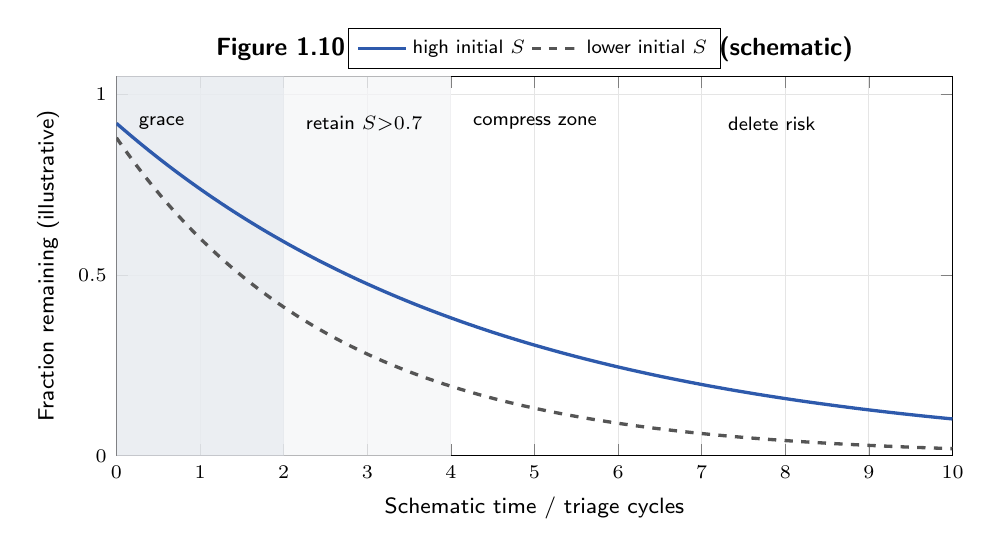
\begin{tikzpicture}
\begin{axis}[
  width=12.2cm, height=6.4cm,
  xmin=0, xmax=10,
  ymin=0, ymax=1.05,
  xlabel={\footnotesize Schematic time / triage cycles},
  ylabel={\footnotesize Fraction remaining (illustrative)},
  grid=major,
  grid style={DarsGray!15},
  tick label style={font=\scriptsize\sffamily},
  label style={font=\footnotesize\sffamily},
  title={\small\sffamily\bfseries Figure 1.10 --- Survival under janitor policy (schematic)},
  title style={yshift=-0.15cm},
  legend style={font=\scriptsize\sffamily, at={(0.5,1.02)}, anchor=south, legend columns=-1},
]

  % shaded policy bands (vertical regions as annotation)
  \fill[DarsLight, opacity=0.85] (axis cs:0,0) rectangle (axis cs:2,1.05);
  \fill[DarsBand, opacity=0.75] (axis cs:2,0) rectangle (axis cs:4,1.05);
  \node[font=\scriptsize\sffamily, anchor=west] at (axis cs:0.15,0.92) {grace};
  \node[font=\scriptsize\sffamily, anchor=west] at (axis cs:2.15,0.92) {retain $S{>}0.7$};
  \node[font=\scriptsize\sffamily, anchor=west] at (axis cs:4.15,0.92) {compress zone};
  \node[font=\scriptsize\sffamily, anchor=west] at (axis cs:7.2,0.92) {delete risk};

  \addplot[very thick, DarsAccent, smooth, domain=0:10, samples=80] {0.92*exp(-0.22*x)};
  \addplot[very thick, DarsGray, dashed, smooth, domain=0:10, samples=80] {0.88*exp(-0.38*x)};
  \legend{high initial $S$, lower initial $S$}

\end{axis}
\end{tikzpicture}
\end{document}
